%
%  untitled
%
%  Created by Dean Freestone on 2010-07-06.
%  Copyright (c) 2010 . All rights reserved.
%
\documentclass[]{article}

% Use utf-8 encoding for foreign characters
\usepackage[utf8]{inputenc}

% Setup for fullpage use
\usepackage{fullpage}

% Uncomment some of the following if you use the features
%
% Running Headers and footers
%\usepackage{fancyhdr}

% Multipart figures
%\usepackage{subfigure}

% More symbols
%\usepackage{amsmath}
%\usepackage{amssymb}
%\usepackage{latexsym}

% Surround parts of graphics with box
\usepackage{boxedminipage}

% Package for including code in the document
\usepackage{listings}

% If you want to generate a toc for each chapter (use with book)
\usepackage{minitoc}

% This is now the recommended way for checking for PDFLaTeX:
\usepackage{ifpdf}

\usepackage{amsmath,amssymb,amsfonts,epsfig} % Typical maths resource packages

%\newif\ifpdf
%\ifx\pdfoutput\undefined
%\pdffalse % we are not running PDFLaTeX
%\else
%\pdfoutput=1 % we are running PDFLaTeX
%\pdftrue
%\fi

\ifpdf
\usepackage[pdftex]{graphicx}
\else
\usepackage{graphicx}
\fi
\title{Patient-Specific Neural Field Model}
\author{Parham Aram, Dean Freestone, Kenneth Scerri, Michael Dewar,\\
 Jacob Donoghue, Sydney Cash, David Grayden and Visakan Kadirkamanathan  }

\date{2010-07-06}

\begin{document}

\ifpdf
\DeclareGraphicsExtensions{.pdf, .jpg, .tif}
\else
\DeclareGraphicsExtensions{.eps, .jpg}
\fi

\maketitle


\begin{abstract}
	
	\begin{itemize}
		\item Background
		\item Method
		\item Result
		\item Conclusion
	\end{itemize}
\end{abstract}

\section{Introduction}
\begin{itemize}
	\item Understanding of macroscopic neurodynamics
	\item Neural field model
	\item Improvements in electrode technology with great spatiotemporal resolution
\end{itemize}

\section{Method}

\subsection{Data Collection}
\begin{itemize}
	\item Show medical imaging
	\item Show LFP Data (background, seizure, post-seizure)
	\item Show spectral properties of LFPs
\end{itemize}

\begin{figure}[!ht]
\begin{center}
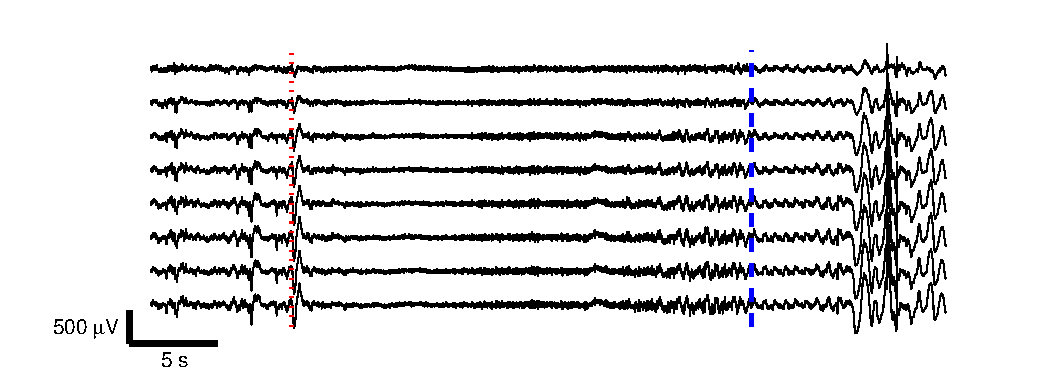
\includegraphics{./Figures/LFPs.eps}
\end{center}
\caption{{\bf Local Field Potentials}. Data recorded from the first five channels of the array. The red dotted line indicates the seizure onset and the blue dashed line indicates the seizure end.}
\label{fig:TimeSeries}
\end{figure}

\begin{figure}[!ht]
\begin{center}
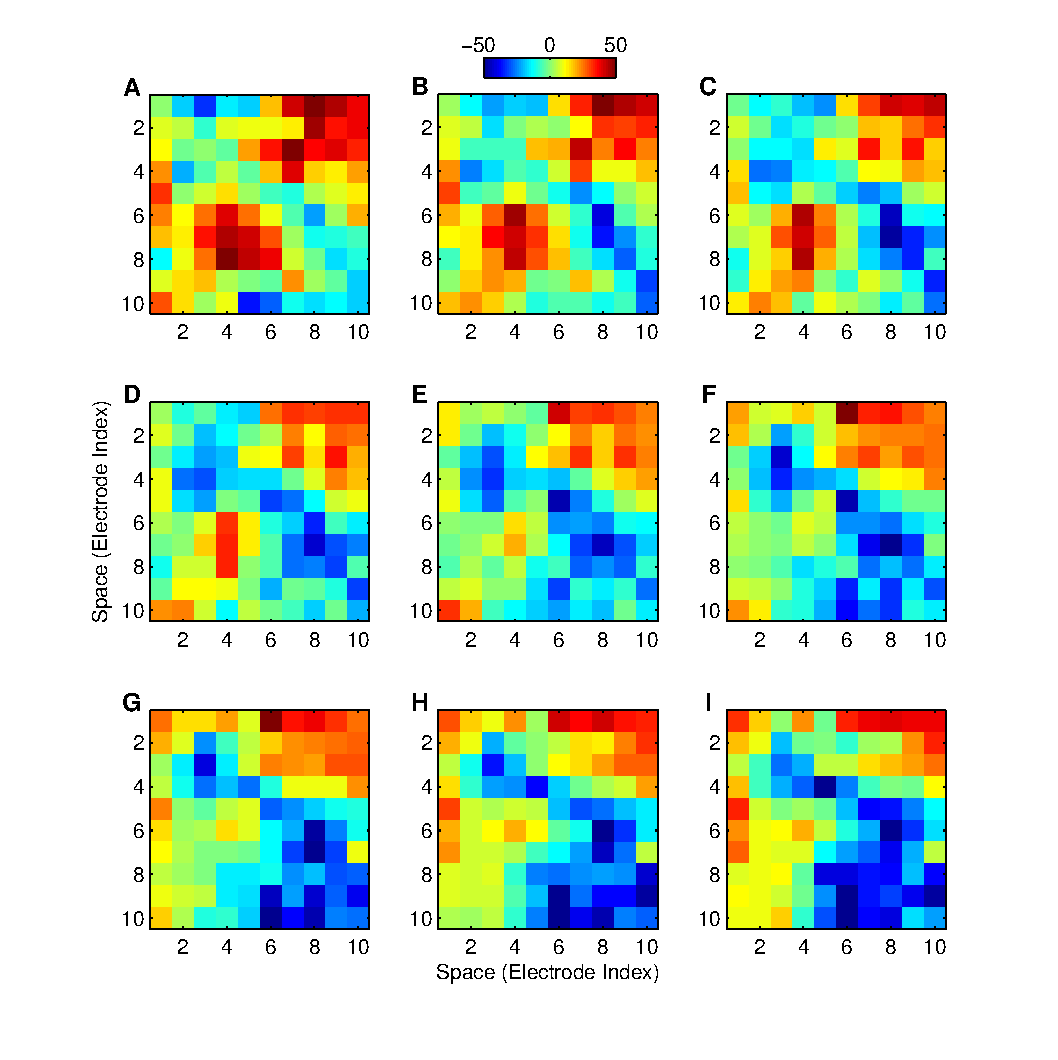
\includegraphics{./Figures/FieldObservations.eps}
\end{center}
\caption{{\bf Snap-shots of the spatial aspects of the observed field}. The snap-shots are ordered from A to I forming a consecutive sequence spaced 2.5~ms apart starting at 34.024s}
\label{fig:FieldObserations}
\end{figure}

\begin{figure}[!ht]
\begin{center}
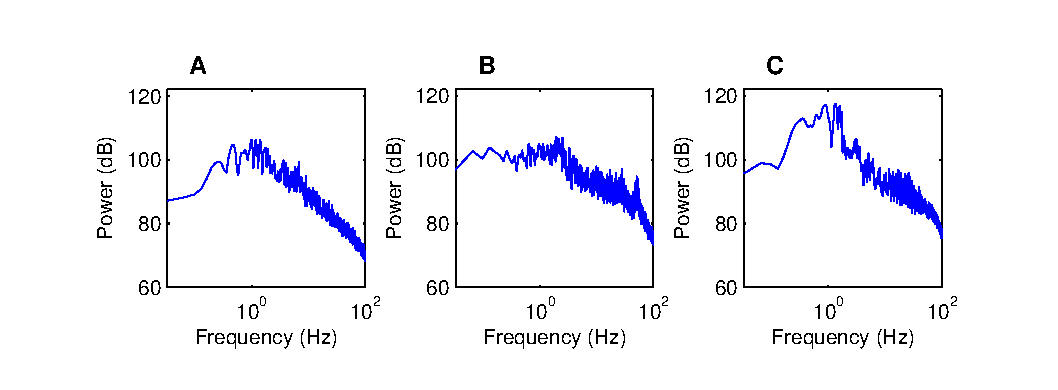
\includegraphics{./Figures/TemporalFreq.eps}
\end{center}
\caption{{\bf Spectra from local field potential recordings}. A. Pre-seizure observations. B. Seizure observations. C. Post-seizure observations.}
\label{fig:TemporalFreqObservation}
\end{figure}

\subsection{Frequency Analysis}
\begin{itemize}
	\item Create 2D FT of observations to estimate bandwidth
\end{itemize}

\begin{figure}[!ht]
\begin{center}
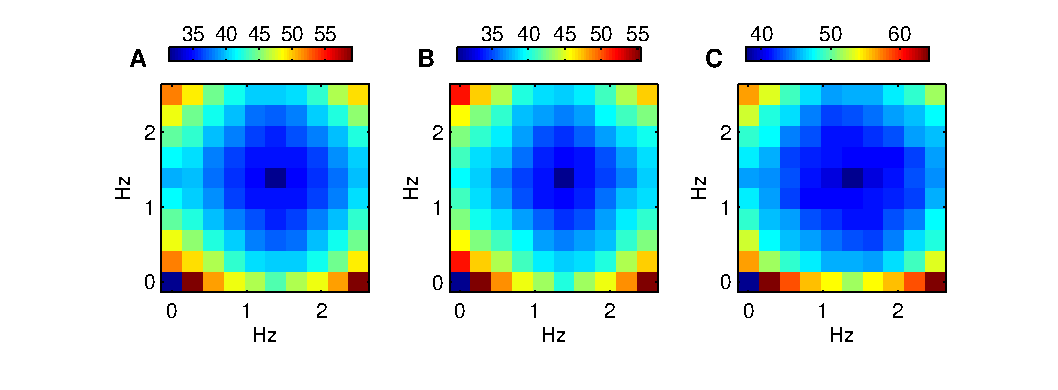
\includegraphics{./Figures/SpatialFreq.eps}
\end{center}
\caption{{\bf Spatial frequency analysis of the observed neural field}. A. Pre-seizure observations. B. Seizure observations. C. Post-seizure observations.}
\label{fig:SpatialFreqObservation}
\end{figure}

\begin{figure}[!ht]
\begin{center}
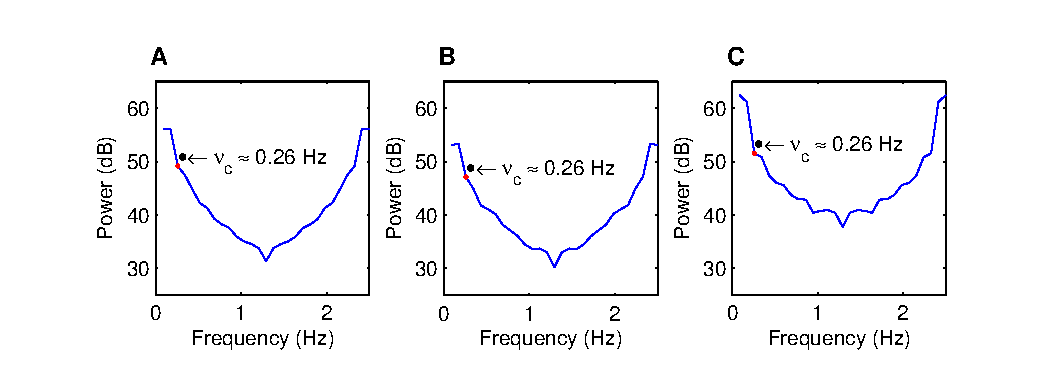
\includegraphics{./Figures/SpatialFreqCrossSection.eps}
\end{center}
\caption{{\bf Diagonal cross-section of the spatial frequency plots of the observed neural field}. A. Pre-seizure observations. B. Seizure observations. C. Post-seizure observations.}
\label{fig:SpatialFreqObservation}
\end{figure}

\subsection{Estimating Support For Connectivity Kernel}
\begin{figure}[!ht]
\begin{center}
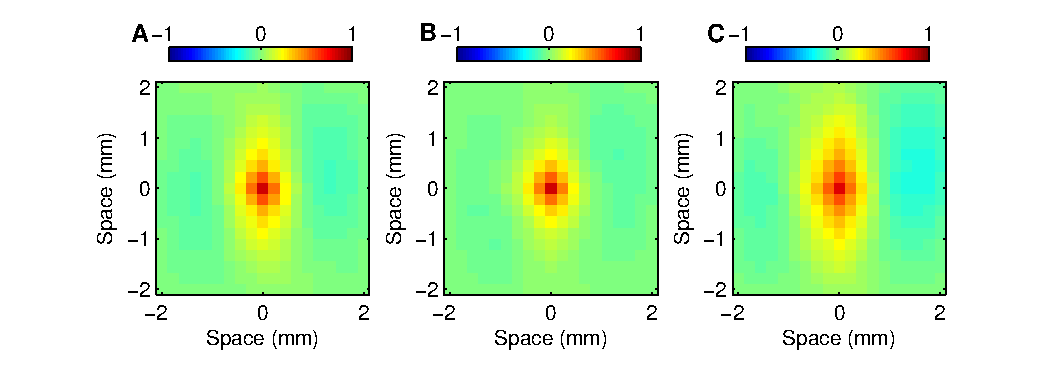
\includegraphics[angle=-90]{./Figures/CrossCorr2D.eps}
\end{center}
\caption{{\bf Mean cross-correlations between consecutive observations of the neural field}. Note: The correlations are normalised such that the maximum value is one. A. Pre-seizure observation correlations. B. Seizure observation correlations. C. Post-seizure observation correlations.}
\label{fig:SpatialFreqObservation}
\end{figure}

\subsection{Pre-processing}
\begin{itemize}
	\item Identification and removal of bad channels
	\item Common average reference (CAR) montage 
	\item Low-pass filter data, with cut-off at 100~Hz
	\item Decimate data from 30~kHz to 5~kHz temporal sampling
	\item Spatially interpolate missing data to facilitate spatial frequency analysis
\end{itemize}
\subsection{Estimation Algorithm}
The state space model is given by
\begin{equation}
 \mathbf x_{t+1}=\boldsymbol\Theta q(\mathbf x_t)+\xi \mathbf x_t+\boldsymbol e_t(\mathbf r)
\end{equation}
\begin{equation}
 \mathbf y_t=\mathbf C \mathbf x_t+\boldsymbol \epsilon_t
\end{equation}
where $\boldsymbol\Theta$ is an $n_x \times n_x$ block matrix where each block matrix is of dimension $ 1\times n_{\theta}$ defined as
\begin{equation}
\boldsymbol \Theta_{i,j}=\left\lbrace  \begin{array}{cc}
\boldsymbol \theta^\top &i=j \\
\mathbf 0_{1 \times n_{\theta}}& i\neq j  
 \end{array}\right. 
\end{equation}
and the non-linear map $q(.)$ is defined as
\begin{equation}\label{eq:QmatrixForSigmapoints}
	q(\mathbf{x}_t) \triangleq T_s\boldsymbol{\Gamma}^{-1} \int_\Omega \boldsymbol{\Lambda}(\mathbf{r}') f(\boldsymbol{\phi}^{\top}(\mathbf{r}')\mathbf{x}_t) d\mathbf{r}'.
\end{equation}
where $\boldsymbol{\Lambda}(\mathbf{r}')  $ is an $n_x \times 1$ block vector with each block of dimension $n_{\theta} \times 1 $
\begin{equation}\label{eq:DefPsi}
\boldsymbol{\Lambda}(\mathbf{r}')=\begin{bmatrix}\boldsymbol \lambda_1(\mathbf r')\\\boldsymbol \lambda_2(\mathbf r')\\ \vdots \\ \boldsymbol \lambda_{n_{x}}(\mathbf r') \end{bmatrix}_{n_x \times 1}
\end{equation}
and where
\begin{equation}
\boldsymbol \lambda_i(\mathbf r') =\begin{bmatrix} \phi_i\ast \psi_1(\mathbf r') \\ \phi_i\ast \psi_2 (\mathbf r') \\ \vdots \\ \phi_i\ast \psi_{n_{\theta}}(\mathbf r') \end{bmatrix}_{n_{\theta} \times 1}
\end{equation}
As a result $q(\mathbf x_t)$ is an $n_x \times 1$ block vector and each block is $n_{\theta} \times 1$. It should be noted that $\boldsymbol\Theta q(\mathbf x_t)$ is an $n_x \times 1$ vector.
$ \boldsymbol e_t(\mathbf r)\sim \mathcal N(\mathbf 0,\boldsymbol\Sigma_e(\mathbf r,\mathbf r'))$ is temporally white and spatially colored disturbance and  $\boldsymbol\epsilon_t\sim \mathcal N(\mathbf 0,\boldsymbol\Sigma_{\epsilon})$ is a white noise process.
\subsection*{$\mathcal Q$-function}
Expanding the joint distribution $p(\mathbf X,\mathbf Y;\boldsymbol \theta,\xi)$ we have
\begin{equation}
 p(\mathbf X,\mathbf Y;\boldsymbol \theta,\xi)=\prod_{t=1}^{T} p(\mathbf y_t|\mathbf x_t)p(\mathbf x_t|\mathbf x_{t-1};\boldsymbol \theta, \xi)p(\mathbf x_0)
\label{eq:jointdistribution}
\end{equation}
The $\mathcal Q$-function can be written in terms of its component as shown in (\ref{eq:jointdistribution})
\begin{eqnarray}
 \mathcal Q(\boldsymbol \theta,\xi,\boldsymbol\theta',\xi')&=&\mathbf E_{\boldsymbol (\theta',\xi')}[\ln p(\mathbf X,\mathbf Y;\boldsymbol \theta,\xi)]\nonumber\\
&=&\mathbf E_{\boldsymbol (\theta',\xi')}[\sum_{t=1}^{T}\ln p(\mathbf y_t|\mathbf x_t)+\sum_{t=1}^{T}\ln p(\mathbf x_t|\mathbf x_{t-1};\boldsymbol \theta)+\sum_{t=1}^{T}\ln p(\mathbf x_0)]
\end{eqnarray}
$p(\mathbf y_t|\mathbf x_t)$ and $p(\mathbf x_0)$ are not functions of parameter therefore $\mathcal Q$-function can be rewritten as
\begin{equation}
\mathcal Q(\boldsymbol \theta,\xi,\boldsymbol\theta',\xi')=\mathbf E_{(\theta',\xi')}[\sum_{t=1}^{T}\ln p(\mathbf x_t|\mathbf x_{t-1};\boldsymbol \theta ,\xi)]+\textrm{const}
\end{equation}
The Gaussian distribution of the disturbance, $e_t(\mathbf r)\sim \mathcal N(\mathbf 0,\boldsymbol\Sigma_e(\mathbf r,\mathbf r'))$ results into the following conditional distribution of the state at $t+1$
\begin{equation}
 p(\mathbf x_{t+1} | \mathbf x_t;\boldsymbol\theta,\xi)=ce^{-(\mathbf x_{t+1}-\boldsymbol\Theta q(\mathbf  x_t)-\xi  \mathbf x_t)^\top\boldsymbol\Sigma_e^{-1}(\mathbf x_{t+1}-\boldsymbol\Theta q( \mathbf x_t)-\xi \mathbf  x_t)}
\end{equation}
where c is the normalising constant. Taking $\log$ we get
\begin{equation}
 \ln p(\mathbf x_{t+1} |\mathbf x_t;\boldsymbol\theta,\xi)=\ln c -(\mathbf x_{t+1}^\top-q^\top(\mathbf x_t)\boldsymbol\Theta^\top -\xi  \mathbf x_t^\top)\boldsymbol\Sigma_e^{-1}(\mathbf x_{t+1}-\boldsymbol\Theta q(\mathbf x_t)-\xi \mathbf x_t)
\end{equation}
\begin{eqnarray}
 \ln p(\mathbf x_{t+1} | \mathbf x_t;\boldsymbol\theta, \xi)&=&\ln c-[\mathbf x_{t+1}^\top\boldsymbol\Sigma_e^{-1}\mathbf x_{t+1}-\mathbf x_{t+1}^\top\boldsymbol\Sigma_e^{-1}\boldsymbol\Theta q(\mathbf x_t)-\xi \mathbf x_{t+1}^\top\boldsymbol\Sigma_e^{-1}\mathbf x_t \nonumber \\
&&- q^\top(\mathbf x_t)\boldsymbol\Theta^\top\boldsymbol\Sigma_e^{-1}\mathbf x_{t+1}+q^\top(\mathbf x_t)\boldsymbol\Theta^\top\boldsymbol\Sigma_e^{-1}\boldsymbol\Theta q(\mathbf x_t)+\xi q^\top(\mathbf x_t)\boldsymbol\Theta^\top \boldsymbol\Sigma_e^{-1}\mathbf x_t \nonumber\\
&&-\xi \mathbf x_t^\top\boldsymbol\Sigma_e^{-1}\mathbf x_{t+1}+\xi  \mathbf  x_t^\top\boldsymbol\Sigma_e^{-1}\boldsymbol\Theta q(\mathbf x_t)+\xi^2\mathbf x_t^\top\boldsymbol\Sigma_e^{-1}\mathbf x_t]
\end{eqnarray}
\begin{eqnarray}\label{eq:Qfunctioninter}
  \ln p(\mathbf x_{t+1} | \mathbf x_t;\boldsymbol\theta,\xi)&=&\ln c-\mathbf x_{t+1}^\top\boldsymbol\Sigma_e^{-1}\mathbf x_{t+1}+2\mathbf x_{t+1}^\top\boldsymbol\Sigma_e^{-1}\boldsymbol\Theta q( \mathbf x_t)+2\xi \mathbf x_{t+1}^\top\boldsymbol\Sigma_e^{-1}\mathbf x_t\nonumber \\
&&-q^\top(\mathbf x_t)\boldsymbol\Theta^\top \boldsymbol\Sigma_e^{-1}\boldsymbol\Theta q(\mathbf x_t)-2\xi \mathbf x_t^\top\boldsymbol\Sigma_e^{-1}\boldsymbol\Theta q(\mathbf x_t)-\xi^2\mathbf x_t^\top\boldsymbol\Sigma_e^{-1}\mathbf x_t
\end{eqnarray}
taking trace and using invariant cyclic permutations property of the trace this distribution can be written as 
 \begin{eqnarray}
   \ln p(x_{t+1} | \mathbf x_t;\boldsymbol\theta,\xi)&=&\ln c-\mathbf x_{t+1}^\top\boldsymbol\Sigma_e^{-1}\mathbf x_{t+1}+2 tr \left\lbrace  \boldsymbol\Theta q( \mathbf x_t)\mathbf x_{t+1}^\top\boldsymbol\Sigma_e^{-1}\right\rbrace  +2 \xi tr\left\lbrace \mathbf x_t\mathbf x_{t+1}^\top\boldsymbol\Sigma_e^{-1}\right\rbrace  \nonumber\\
 &&-tr \left\lbrace \boldsymbol\Theta q(\mathbf x_t)q^\top(\mathbf x_t)\boldsymbol\Theta^\top \boldsymbol\Sigma_e^{-1}\right\rbrace  -2\xi tr \left\lbrace \boldsymbol\Theta q(\mathbf x_t)  \mathbf x_t^\top\boldsymbol\Sigma_e^{-1} \right\rbrace -\xi^2 tr \left\lbrace\mathbf x_t\mathbf x_t^\top\boldsymbol\Sigma_w^{-1} \right\rbrace  \nonumber
 \end{eqnarray} 
taking the expected value is leading to the following  $\mathcal Q$-function
\begin{eqnarray}
 \mathcal Q(\boldsymbol \theta,\xi,\boldsymbol\theta',\xi')&=&\beta+2 tr\left\lbrace \boldsymbol\Theta\Xi_2\boldsymbol\Sigma_e^{-1}\right\rbrace +2\xi tr \left\lbrace  \Xi_0\boldsymbol\Sigma_e^{-1}\right\rbrace  \nonumber \\
&-&tr \left\lbrace\boldsymbol\Theta\Xi_4 \boldsymbol\Theta^\top\boldsymbol\Sigma_e^{-1}\right\rbrace -2\xi tr \left\lbrace \boldsymbol\Theta\Xi_3\boldsymbol\Sigma_e^{-1}\right\rbrace  \nonumber \\
&-&\xi^2 tr \left\lbrace \Xi_1\boldsymbol\Sigma_e^{-1}\right\rbrace  \nonumber
\end{eqnarray}
where  $\beta= \sum_{t=1}^T\mathbf E_{(\theta',\xi)}[ \ln c-\mathbf x_{t+1}^\top\boldsymbol\Sigma_w^{-1}\mathbf x_{t+1}]$ is constant with respect to the parameters and will disapear by differentiation and 
\begin{equation}
 \Xi_0=\sum_{t=1}^T\mathbf E_{(\theta',\xi')}[\mathbf x_t\mathbf x_{t+1}^\top] \quad \Xi_1=\sum_{t=1}^T\mathbf E_{(\theta',\xi')}[\mathbf x_t\mathbf x_t^\top]
\end{equation}
Other terms can be approximated by linearising $q(\mathbf x)$ and taking the first-order truncated  Taylor-series expansion around the mean of the state at each time instant, i.e. 
\begin{equation}\label{eq:qTaylor}
 q(\mathbf x_t)\approx q(\hat{\mathbf x}_t)+\nabla^\top q (\hat{\mathbf x}_t)(\mathbf x_t -\hat{\mathbf x}_t)
\end{equation}
where
\begin{equation}
\nabla q=\begin{bmatrix}\frac{\delta q}{\delta x_1} \mid_{{\mathbf x}_t=\mathbf{\hat x}_t} &\frac{\delta q}{\delta x_2} \mid_{{\mathbf x}_t=\mathbf{\hat x}_t}& \dots &\frac{\delta q}{\delta x_n} \mid_{{\mathbf x}_t=\mathbf{\hat x}_t}\end{bmatrix}^\top
\end{equation}
therefore
\begin{equation}
 \Xi_2=\sum_{t=1}^{T}\mathbf E_{(\theta',\xi')}[q(\mathbf x_t)\mathbf x_{t+1}^\top ], \quad \mathbf E_{(\theta',\xi')}[q(\mathbf x_t)\mathbf x_{t+1}^\top ]\approx q(\mathbf{ \hat x}_t)\mathbf{ \hat x}_{t+1}^\top+\nabla^\top q(\mathbf{ \hat x}_t)\mathbf M_t
\end{equation}
\begin{equation}
 \Xi_3=\sum_{t=1}^{T}\mathbf E_{(\theta',\xi')}[q(\mathbf x_t)\mathbf x_{t}^\top ], \quad \mathbf E_{(\theta',\xi')}[q(\mathbf x_t)\mathbf x_{t}^\top ]\approx q(\mathbf{ \hat x}_t)\mathbf{ \hat x}_{t}^\top+\nabla^\top q(\mathbf{ \hat x}_t)\mathbf P_t
\end{equation}
\begin{equation}
 \Xi_4=\sum_{t=1}^{T}\mathbf E_{(\theta',\xi')}[q(\mathbf x_t)q^\top(\mathbf x_t) ], \quad \mathbf E_{(\theta',\xi')}[q(\mathbf x_t)q^\top(\mathbf x_t) ] \approx q(\mathbf{ \hat x}_t)q^\top(\mathbf{ \hat x}_t)+\nabla^\top q(\mathbf{ \hat x}_t)\mathbf P_t\nabla q(\mathbf{ \hat x}_t)
\end{equation}
we rewrite the $\mathcal Q$-function as
\begin{eqnarray}\label{eq:rewrittenQ}
 \mathcal Q(\boldsymbol \theta,\xi,\boldsymbol\theta',\xi')&=&\beta+2  \sum_{i,j,k=1}^{n_x}[\boldsymbol\Theta]_{i,j}[\Xi_2]_{j,k}[\boldsymbol\Sigma_e^{-1}]_{k,i} +2\xi tr \left\lbrace  \Xi_0\boldsymbol\Sigma_e^{-1}\right\rbrace  \nonumber \\
&-& \sum_{i,j,k,l=1}^{n_x}[\boldsymbol\Theta]_{i,j}[\Xi_4]_{j,k}[ \boldsymbol\Theta^\top]_{k,l}[\boldsymbol\Sigma_e^{-1}]_{l,i} -2\xi \sum_{i,j,k=1}^{n_x}[\boldsymbol\Theta]_{i,j}[\Xi_3]_{j,k}[\boldsymbol\Sigma_e^{-1}]_{k,i}  \nonumber \\
&-&\xi^2 tr \left\lbrace \Xi_1\boldsymbol\Sigma_e^{-1}\right\rbrace  
\end{eqnarray}
we can simplify \eqref{eq:rewrittenQ} by noting that $[\boldsymbol \Theta]_{i,j}=\mathbf 0 \quad i \neq j$ 

\begin{equation}
 \mathcal Q(\boldsymbol \theta,\xi,\boldsymbol\theta',\xi')=\beta +2\xi r_0 -\xi^2 r_1 +2 \boldsymbol\theta^\top \mathbf r_2-2\xi \boldsymbol\theta^\top \mathbf r_3  -\boldsymbol\theta^\top\mathbf R_4\boldsymbol\theta 
\end{equation}
where 
\begin{equation}
 r_0=tr \left\lbrace  \Xi_0\boldsymbol\Sigma_e^{-1}\right\rbrace   \quad r_1=tr \left\lbrace \Xi_1\boldsymbol\Sigma_e^{-1}\right\rbrace \quad
 \mathbf r_2=tr\left\lbrace \Xi_2\boldsymbol\Sigma_e^{-1}\right\rbrace \quad  \mathbf r_3= tr \left\lbrace \Xi_3\boldsymbol\Sigma_e^{-1}\right\rbrace \quad \mathbf R_4= tr \left\lbrace\Xi_4 \boldsymbol\Sigma_e^{-1}\right\rbrace\nonumber 
\end{equation}

differentiate with respect to $\boldsymbol\theta$ and equating to zero we have
\begin{eqnarray}
\frac{\delta \mathcal Q}{\delta \boldsymbol \theta}=2\mathbf r_2^\top-2\xi \mathbf r_3^\top-2\boldsymbol \theta^\top\mathbf R_4^\top=0
\end{eqnarray}
therefore
\begin{equation}\label{eq:thetasolution}
 \boldsymbol \theta=\mathbf R_4^{-1}(\mathbf r_2-\xi\mathbf r_3)
\end{equation}
differentiate with respect to $\xi$ we have
\begin{equation}
 \frac{\delta \mathcal Q}{\delta \xi}=+2r_0-2\xi r_1-2\boldsymbol\theta^\top\mathbf r_3=0
\end{equation}
and we get
\begin{equation}\label{eq:xisolution}
 \xi=\frac{1}{r_1}(r_0- \boldsymbol \theta^\top \mathbf r_3)
\end{equation}
substituting \eqref{eq:thetasolution} in \eqref{eq:xisolution} we get
\begin{eqnarray}
\xi=\frac{r_0-r'_0}{r_1-r'_1}
\end{eqnarray}
where
\begin{equation}
 r'_0=\mathbf r_2^\top \mathbf R_4^{-\top}\mathbf r_3 \quad r'_1=\mathbf r_3^\top \mathbf R_4^{-\top}\mathbf r_3
\end{equation}
and subsequently
\begin{equation}
 \boldsymbol \theta=\mathbf R_4^{-1}(\mathbf r_2+\frac{r'_0-r_0}{r_1-r'_1} \mathbf r_3)
\end{equation}
\subsection*{Discussion}
The second derivative of the $\mathcal Q$-function with respect to $\xi$ is given by
\begin{equation}
 \frac{\delta^2 \mathcal Q}{\delta \xi^2}=-2 r_1 \quad r_1=tr \left\lbrace \Xi_1\boldsymbol\Sigma_e^{-1}\right\rbrace
\end{equation}
$\Xi_1 $ is positive definite if the state vector is persistently excited and the covariance matrix $\boldsymbol\Sigma_w^{-1}$ is also positive definite therefore the trace of $\Xi_1\boldsymbol\Sigma_w^{-1}$ is guaranteed to be positive so the second derivative is negative and represents a maximum of $\mathcal Q$-function.\\
The second derivative of the $\mathcal Q$-function with respect to $\boldsymbol \theta$ is given by
\begin{equation}
 \frac{\delta^2 \mathcal Q}{\delta \boldsymbol\theta^2}=-2\mathbf R_4 \quad \mathbf R_4= tr \left\lbrace\Xi_4 \boldsymbol\Sigma_e^{-1}\right\rbrace
\end{equation}
$\mathbf R_4$ is positive definite and invertible and the second derivative is negative definite and represents a maximum of $\mathcal Q$- function.
\subsection*{Summary of the M-step}
\begin{eqnarray}
\xi=\frac{r_0-r'_0}{r_1-r'_1}
 \quad  \boldsymbol \theta=\mathbf R_4^{-1}(\mathbf r_2+\frac{r'_0-r_0}{r_1-r'_1} \mathbf r_3)
\end{eqnarray}
where
\begin{eqnarray}
 r_0&=&tr \left\lbrace  \Xi_0\boldsymbol\Sigma_e^{-1}\right\rbrace \quad r_1=tr \left\lbrace \Xi_1\boldsymbol\Sigma_e^{-1}\right\rbrace\nonumber \\
r'_0&=&\mathbf r_2^\top \mathbf R_4^{-\top}\mathbf r_3  \quad r'_1=\mathbf r_3^\top \mathbf R_4^{-\top}\mathbf r_3 \nonumber \\
\nonumber \\
 \mathbf r_2&=&tr\left\lbrace \Xi_2\boldsymbol\Sigma_e^{-1}\right\rbrace \quad \mathbf r_3= tr \left\lbrace \Xi_3\boldsymbol\Sigma_e^{-1}\right\rbrace \nonumber \\ 
 \mathbf R_4&=& tr \left\lbrace\Xi_4 \boldsymbol\Sigma_e^{-1}\right\rbrace\nonumber 
\end{eqnarray}

\begin{equation}
 \Xi_0=\sum_{t=1}^T\mathbf E_{(\theta',\xi')}[\mathbf x_t\mathbf x_{t+1}^\top] \quad \Xi_1=\sum_{t=1}^T\mathbf E_{(\theta',\xi')}[\mathbf x_t\mathbf x_t^\top]
\end{equation}
\begin{equation}
 \Xi_2=\sum_{t=1}^{T}\mathbf E_{(\theta',\xi')}[q(\mathbf x_t)\mathbf x_{t+1}^\top ], \quad \mathbf E_{(\theta',\xi')}[q(\mathbf x_t)\mathbf x_{t+1}^\top ]=q(\mathbf{ \hat x}_t)\mathbf{ \hat x}_{t+1}^\top+\nabla^\top q(\mathbf{ \hat x}_t)\mathbf M_t
\end{equation}
\begin{equation}
 \Xi_3=\sum_{t=1}^{T}\mathbf E_{(\theta',\xi')}[q(\mathbf x_t)\mathbf x_{t}^\top ], \quad \mathbf E_{(\theta',\xi')}[q(\mathbf x_t)\mathbf x_{t}^\top ]=q(\mathbf{ \hat x}_t)\mathbf{ \hat x}_{t}^\top+\nabla^\top q(\mathbf{ \hat x}_t)\mathbf P_t
\end{equation}
\begin{equation}
 \Xi_4=\sum_{t=1}^{T}\mathbf E_{(\theta',\xi')}[q(\mathbf x_t)q^\top(\mathbf x_t) ], \quad \mathbf E_{(\theta',\xi')}[q(\mathbf x_t)q^\top(\mathbf x_t) ]=q(\mathbf{ \hat x}_t)q^\top(\mathbf{ \hat x}_t)+\nabla^\top q(\mathbf{ \hat x}_t)\mathbf P_t\nabla q(\mathbf{ \hat x}_t)
\end{equation}

\section{Results}
\begin{itemize}
	\item Will show parameter distributions
	\item Will show parameter changes over time through the seizure
\end{itemize}

\section{Discussion}
\begin{itemize}
	\item  
\end{itemize}

\bibliographystyle{plain}
\bibliography{}
\end{document}
